\documentclass[conference]{IEEEtran}
\IEEEoverridecommandlockouts
\usepackage{cite}
\usepackage{amsmath,amssymb,amsfonts}
\usepackage{graphicx}
\usepackage{booktabs}
\usepackage{url}
\def\BibTeX{{\rm B\kern-.05em{\sc i\kern-.025em b}\kern-.08em T\kern-.1667em\lower.7ex\hbox{E}\kern-.125emX}}

\begin{document}

\title{Who Does the Recommender Serve? A Fairness Audit and\\
Mitigation of Demographic Bias in Distributed\\
Rating Classification on MovieLens 1M}

\author{
\IEEEauthorblockN{Shahriar Fahim, Rutvik Katkoriya, Mostafizur Rahman, Aliia Rustamova}
\IEEEauthorblockA{\textit{Department of Computer Science} \\
\textit{San Francisco Bay University}\\
Fremont, CA, USA}
}

\maketitle

\begin{abstract}
Rating-prediction models are routinely evaluated on aggregate accuracy, which
hides whether a model serves different demographic groups equally. We audit a
distributed logistic-regression classifier that predicts whether a user rates a
movie highly ($\text{rating}\geq 4$) on the MovieLens 1M dataset, implemented as an
Apache Spark ML pipeline. We first identify and correct a target-leakage flaw in a
common feature recipe---user- and movie-average ratings computed over the full
dataset---which modestly inflated accuracy from $0.723$ to a corrected $0.719$;
correcting it is nonetheless a prerequisite for an honest audit. On the corrected
model, aggregate accuracy of $0.72$ conceals sharply different behavior by protected
attribute: gender disparity is mild (demographic parity difference, DPD, of $0.036$;
disparate impact, DI, of $0.95$), but \emph{age} disparity is substantial
(DPD $=0.146$, DI $=0.80$, at the common four-fifths threshold), with the model
under-selecting items for younger users and over-selecting for older users. We then
evaluate two mitigations. Removing the protected attributes from the feature set
(``fairness through unawareness'') did not help and \emph{worsened} the age gap
(DPD $0.146\rightarrow0.215$), because correlated proxies remain. Per-group
threshold calibration nearly eliminated the gender gap (DPD $\rightarrow 0.001$) at
a negligible accuracy cost ($0.0008$), but, being attribute-specific, left the age
gap unchanged. Our results argue that fairness must be measured per attribute, that
dropping protected features is insufficient, and that leakage-aware evaluation is a
precondition for trustworthy fairness claims.
\end{abstract}

\begin{IEEEkeywords}
algorithmic fairness, recommender systems, Apache Spark, logistic regression,
demographic bias, MovieLens, disparate impact
\end{IEEEkeywords}

\section{Introduction}
Recommender and rating-prediction systems increasingly mediate what content users
see, yet their evaluation is dominated by aggregate accuracy that treats all users
as interchangeable. A model can report strong overall accuracy while systematically
under-serving a demographic subgroup. As machine learning moves into consequential
settings, this gap between aggregate performance and per-group performance has
become central to trustworthy AI \cite{mehrabi2021survey,barocas2016big}.

We study this on a concrete, reproducible artifact: a logistic-regression classifier
predicting the binary target ``high rating'' ($\text{rating}\geq 4$) for a
(user, movie) pair on MovieLens 1M \cite{harper2015movielens}, built as an Apache
Spark ML pipeline \cite{meng2016mllib,zaharia2016spark}. The setting is deliberately
mainstream---logistic regression on MovieLens is a canonical baseline---which makes
it a useful lens on a broader question: \emph{when a standard, well-performing
pipeline is deployed at scale, who does it actually serve?}

Three findings organize the paper. First, the pipeline as originally constructed
suffered from \emph{target leakage}: user- and movie-average rating features were
computed over the entire dataset, including the ratings being predicted. Correcting
this changes accuracy only modestly ($0.723\rightarrow0.719$), but it is a
precondition for an honest audit. Second, the corrected model's aggregate accuracy
of $0.72$ conceals a strong asymmetry between protected attributes: gender disparity
is mild, whereas age disparity is large and sits at the four-fifths disparate-impact
threshold. Third, the intuitive mitigation of removing protected attributes fails
and even worsens the age gap, while a cheap per-group threshold calibration removes
the gender gap almost entirely but does not transfer across attributes.

\textbf{Contributions.}
\begin{itemize}
  \item We identify and correct a target-leakage flaw in a common MovieLens
  feature recipe and quantify its (modest) inflationary effect (\S\ref{sec:leakage},
  \S\ref{sec:audit}).
  \item We conduct a group-fairness audit of a scalable Spark logistic-regression
  classifier across gender and age using DPD, equal-opportunity difference (EOD),
  and disparate impact, showing that a single aggregate score hides an
  attribute-dependent disparity (\S\ref{sec:audit}).
  \item We evaluate two interpretable mitigations and characterize the
  fairness--accuracy tradeoff, including a negative result for feature removal
  (\S\ref{sec:mitigation}).
\end{itemize}

\section{Related Work}\label{sec:related}
\textbf{Fairness definitions.} Dwork et al.\ introduced fairness through awareness
\cite{dwork2012fairness}; Hardt et al.\ proposed equalized odds and equal
opportunity, framing fairness as error-rate parity across groups
\cite{hardt2016equality}; Feldman et al.\ formalized disparate impact and its
removal \cite{feldman2015certifying}. Verma and Rubin catalog these often-conflicting
definitions \cite{verma2018fairness}. We report demographic parity, equal
opportunity, and disparate impact together rather than committing to one.

\textbf{Bias in recommendation.} Ekstrand et al.\ show recommender effectiveness and
evaluation can differ across demographic groups \cite{ekstrand2018all}, and surveys
document how bias enters at data, model, and evaluation stages
\cite{mehrabi2021survey}. Most such work targets ranking or top-$k$ recommendation;
we audit the upstream rating-classification stage, where disparities originate but
are rarely measured.

\textbf{Mitigation.} Mitigations are pre-, in-, or post-processing. Kamiran and
Calders study pre-processing via reweighing \cite{kamiran2012data}; post-processing
adjusts decision thresholds per group \cite{hardt2016equality}. We evaluate one
pre-processing approach (removing sensitive attributes) and one post-processing
approach (per-group thresholds), both interpretable and compatible with a
distributed pipeline. Our feature-removal result is a concrete instance of the
well-known limitation of ``fairness through unawareness'' \cite{dwork2012fairness}.

\textbf{Gap we address.} Prior fairness studies rarely (i) operate on a distributed
big-data engine, (ii) tie the audit to a reproducible interpretable model, and (iii)
control for evaluation artifacts such as target leakage. We address all three.

\section{Methodology}\label{sec:method}
\subsection{Dataset}
MovieLens 1M \cite{harper2015movielens} contains 1{,}000{,}209 ratings from 6{,}040
users on ${\sim}3{,}900$ movies, with per-user gender, age band, and occupation. We
load the ``::''-delimited files with explicit schemas, drop duplicate (user, movie)
ratings, enforce referential integrity, and restrict ratings to $[1,5]$.

\subsection{Task and features}
The target is $y=\mathbb{1}[\text{rating}\geq 4]$. Features are (i) \emph{demographic}
(age, occupation, gender), (ii) \emph{static movie} attributes (release year, movie
age relative to 2000, number of genres), and (iii) \emph{derived interaction}
statistics (user-average rating, movie-average rating, user rating count, movie
popularity). Gender and age serve both as baseline features and as the
\emph{protected attributes} for the audit.

\subsection{Leakage-aware feature construction}\label{sec:leakage}
The derived interaction statistics are label-dependent: a user's average rating over
all their ratings includes the rating being predicted. Computing them over the full
dataset before splitting leaks the test label into test features. We correct this by
performing the 80/20 split \emph{first} (seed 42) and computing all derived
statistics on the training split only, joining them onto test rows and backing off
unseen users/movies to the global training mean ($3.582$). We also build a leaky
reference model (statistics over all data) to measure the effect.

\subsection{Model}
The classifier is a Spark ML \texttt{Pipeline} of
\texttt{VectorAssembler}$\rightarrow$\texttt{StandardScaler}$\rightarrow$
\texttt{LogisticRegression} (max 100 iterations). Logistic regression is chosen for
interpretability: coefficients expose which features drive predictions.

\subsection{Fairness metrics}
For a protected group $g$, let the selection rate be $s_g=P(\hat y=1\mid g)$ and the
true-positive rate $t_g=P(\hat y=1\mid y=1,g)$. We report
\begin{align}
\text{DPD} &= \max_g s_g - \min_g s_g, &
\text{DI}  &= \min_g s_g / \max_g s_g, \\
\text{EOD} &= \max_g t_g - \min_g t_g. &
\end{align}
DPD and DI capture demographic parity; EOD captures equal opportunity. A DI below
$0.8$ is a common disparate-impact threshold \cite{feldman2015certifying}.

\subsection{Mitigations}
\emph{Sensitive-feature removal} retrains with gender and age excluded.
\emph{Per-group threshold calibration} keeps the baseline model but selects a
per-gender decision threshold so each group's selection rate matches the overall
target rate---post-processing toward demographic parity.

\section{Experimental Setup}\label{sec:setup}
Experiments run on a single machine in Spark local mode (\texttt{local[*]}),
Spark 3.5.3, Java 17, Python 3.11. The split uses seed 42; the training set has
$800{,}504$ rows and the test set $199{,}705$. The primary accuracy metric is
overall accuracy; the primary fairness metric is gender DPD, complemented by age
DPD, EOD, and DI. We audit gender (two groups) and age (seven MovieLens bands).
Reported F1 is for the positive class.

\section{Fairness Audit}\label{sec:audit}
\subsection{Leakage correction}
Table~\ref{tab:leakage} reports the leaky and corrected models. Correcting the
leakage moved accuracy from $0.723$ to $0.719$ and positive-class F1 from $0.773$ to
$0.770$. The effect is modest---each average aggregates ${\sim}165$ ratings per user,
so removing one rating barely shifts it---but the correction is methodologically
necessary and all subsequent results use the corrected model.

\begin{table}[t]
\caption{Effect of leakage correction (test set, $n=199{,}705$).}
\label{tab:leakage}
\centering
\begin{tabular}{lcccc}
\toprule
Model & Accuracy & Precision & Recall & F1 \\
\midrule
Leaky (full-data averages) & $0.723$ & $0.731$ & $0.821$ & $0.773$ \\
Corrected (train-only)     & $0.719$ & $0.727$ & $0.817$ & $0.770$ \\
\bottomrule
\end{tabular}
\end{table}

\subsection{Group disparities}
Table~\ref{tab:fairness-base} shows per-gender behavior. The gender gap is mild:
DPD $=0.036$, DI $=0.95$ (well above the $0.8$ threshold), and EOD $=0.007$---by
these measures the model is close to parity across gender. The picture differs
sharply for age. As Fig.~\ref{fig:age} shows, the baseline selection rate rises
almost monotonically with user age, from $0.59$ for the 18--24 band to $0.73$ for
the 56+ band, giving an age DPD of $0.146$, DI of $0.80$ (at the four-fifths
threshold), and EOD of $0.090$. Aggregate accuracy of $0.72$ therefore masks a
substantial age disparity while gender looks benign.

\begin{table}[t]
\caption{Gender fairness of the corrected baseline.}
\label{tab:fairness-base}
\centering
\begin{tabular}{lcccc}
\toprule
Group & $n$ & Sel.\ rate & TPR & Accuracy \\
\midrule
Female & $49{,}177$  & $0.673$ & $0.823$ & $0.710$ \\
Male   & $150{,}528$ & $0.637$ & $0.816$ & $0.722$ \\
\midrule
\multicolumn{5}{l}{Gender: DPD $=0.036$,\ \ EOD $=0.007$,\ \ DI $=0.95$} \\
\multicolumn{5}{l}{Age: \ \ \ \ \ DPD $=0.146$,\ \ EOD $=0.090$,\ \ DI $=0.80$} \\
\bottomrule
\end{tabular}
\end{table}

\begin{figure}[t]
\centering
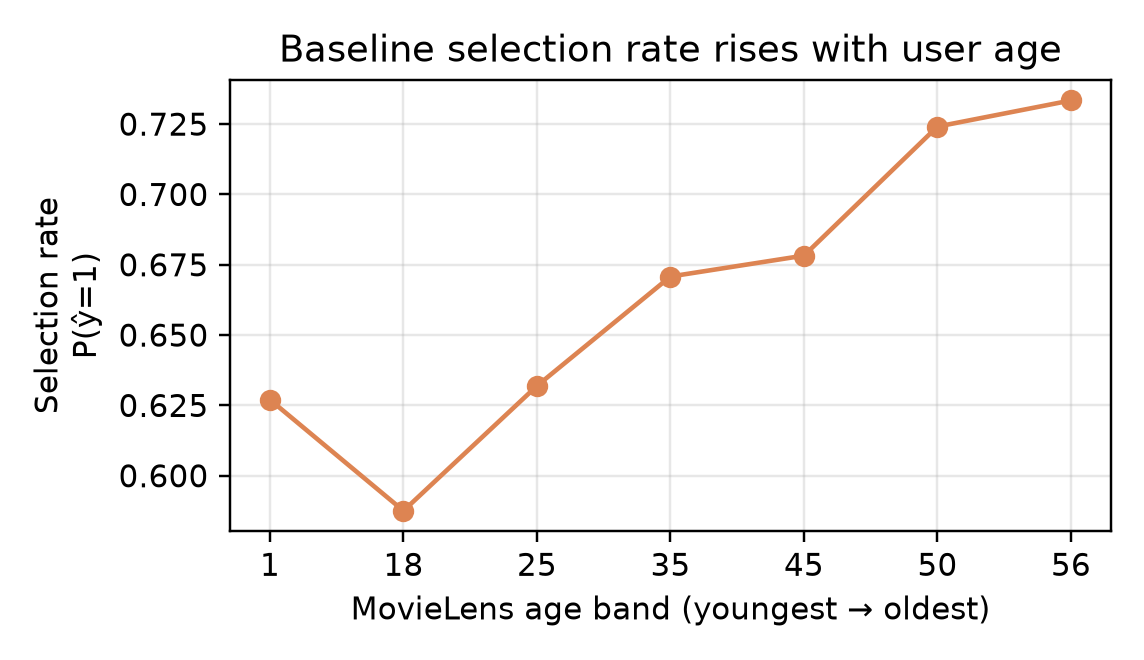
\includegraphics[width=0.92\linewidth]{fig_age.png}
\caption{Baseline selection rate $P(\hat y=1)$ rises with user age band, revealing a
disparity invisible in the aggregate accuracy of $0.72$.}
\label{fig:age}
\end{figure}

\section{Mitigation and Tradeoff}\label{sec:mitigation}
Table~\ref{tab:mitigation} compares the corrected baseline with the two mitigations
on gender, and Fig.~\ref{fig:dpd} shows the DPD for both protected attributes across
all three configurations.

\textbf{Feature removal fails.} Dropping gender and age from the feature set did not
improve gender parity (DPD $0.036\rightarrow0.042$) and \emph{worsened} the age gap
(DPD $0.146\rightarrow0.215$, DI $0.80\rightarrow0.72$). Removing protected
attributes leaves correlated proxies---movie age, genre mix, popularity---through
which the model reconstructs the same disparity, a concrete instance of the limits of
fairness through unawareness \cite{dwork2012fairness}.

\textbf{Per-group thresholds work, but only for the targeted attribute.} Calibrating
a per-gender threshold (male $0.488$, female $0.522$) reduced gender DPD from $0.036$
to $0.001$ (DI $=0.999$) at an accuracy cost of just $0.0008$
($0.719\rightarrow0.718$). Because the thresholds are gender-specific, the age gap
was unchanged (DPD $=0.146$). This illustrates that post-processing is cheap and
effective but must be applied to each attribute one intends to protect.
Fig.~\ref{fig:tradeoff} plots the gender fairness--accuracy tradeoff: per-group
thresholding moves left (fairer) with essentially no vertical (accuracy) drop.

\begin{table}[t]
\caption{Fairness--accuracy comparison on gender.}
\label{tab:mitigation}
\centering
\begin{tabular}{lccc}
\toprule
Configuration & Accuracy & Gender DPD & Gender DI \\
\midrule
Corrected baseline        & $0.719$ & $0.036$ & $0.95$ \\
Sensitive-feature removal & $0.719$ & $0.042$ & $0.94$ \\
Per-group thresholds      & $0.718$ & $0.001$ & $1.00$ \\
\bottomrule
\end{tabular}
\end{table}

\begin{figure}[t]
\centering
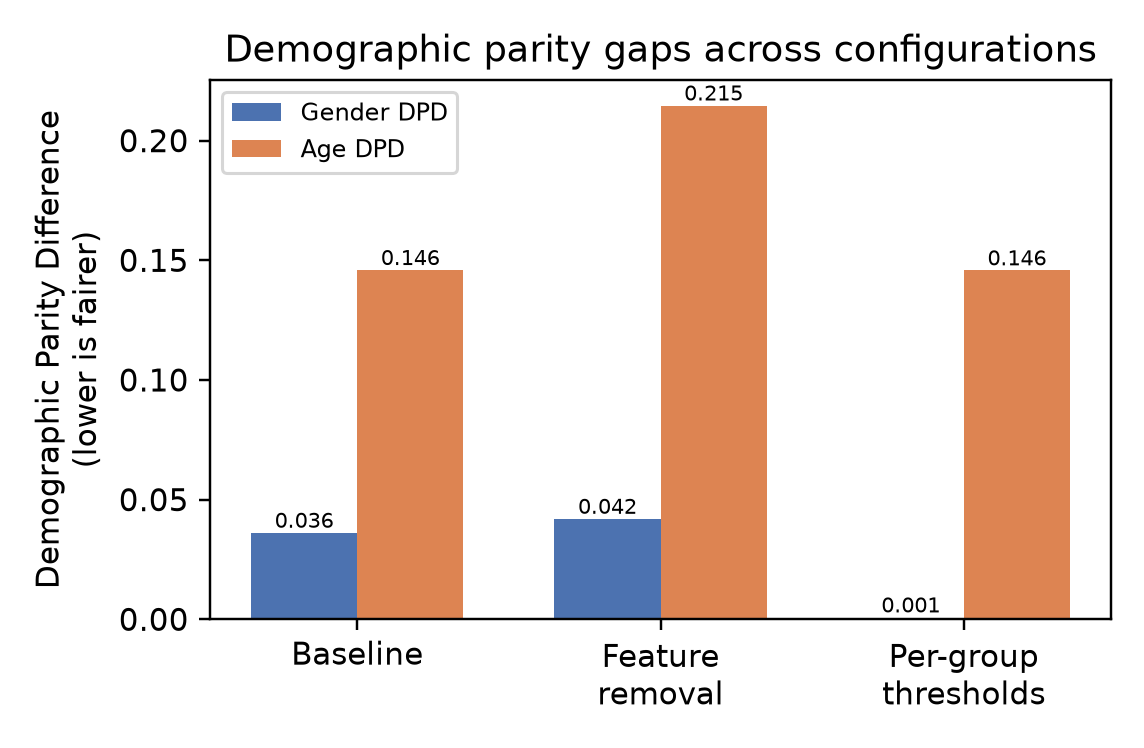
\includegraphics[width=0.92\linewidth]{fig_dpd.png}
\caption{Demographic parity difference by protected attribute across
configurations. Feature removal worsens the age gap; per-group (gender) thresholds
close the gender gap but not the age gap.}
\label{fig:dpd}
\end{figure}

\begin{figure}[t]
\centering
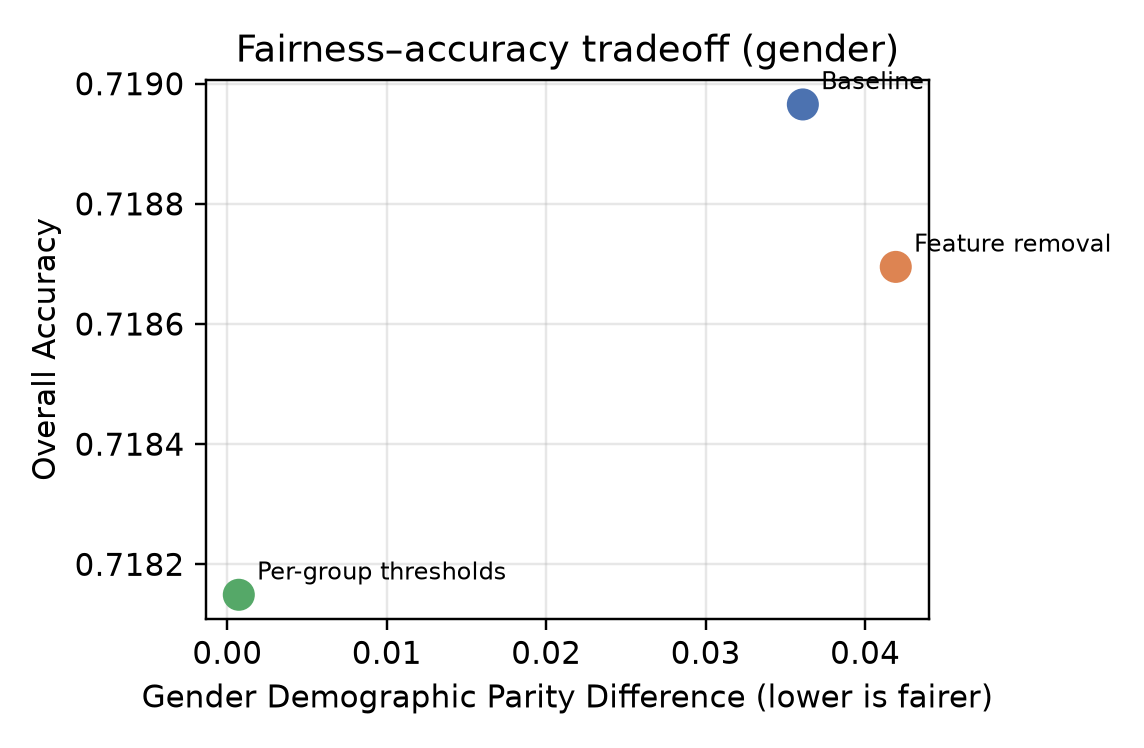
\includegraphics[width=0.86\linewidth]{fig_tradeoff.png}
\caption{Gender fairness--accuracy tradeoff. Per-group thresholding reaches near-zero
DPD at negligible accuracy cost.}
\label{fig:tradeoff}
\end{figure}

\section{Discussion, Limitations, and Threats to Validity}\label{sec:discussion}
\textbf{Interpretation.} The audit yields three transferable lessons: (i) a single
aggregate metric can be simultaneously acceptable and misleading---here gender looks
fair while age does not; (ii) removing protected attributes does not remove bias and
can worsen it via proxies; and (iii) cheap post-processing closes a targeted gap but
does not generalize across attributes.

\textbf{Internal validity.} Results use a single split and seed. We fix seed 42 for
reproducibility but do not report cross-seed variance or significance tests; adding
them is the most important next step before strong claims. Per-group thresholding
also assumes group membership is available at inference, which raises governance
questions of its own.

\textbf{External validity.} MovieLens users are not a representative population, and
gender is a self-reported binary; the audit cannot speak to non-binary users or to
production traffic, and results should not be generalized without re-auditing.

\textbf{Construct validity.} Demographic parity, equal opportunity, and disparate
impact can conflict \cite{verma2018fairness}; we report all three and do not claim
the mitigated model is ``fair'' in an absolute sense---only that specific measured
gaps change as reported.

\section{Conclusion and Future Work}
We audited a scalable, interpretable rating classifier on MovieLens 1M for
demographic fairness. After correcting a target-leakage flaw, we found a mild gender
disparity but a substantial age disparity hidden beneath a $0.72$ aggregate
accuracy; removing protected attributes failed to help and worsened the age gap,
while per-group thresholding closed the gender gap almost for free but did not
transfer to age. Future work includes cross-seed significance testing, stronger
baselines (gradient-boosted trees), age-aware and multi-attribute thresholding,
in-processing fairness constraints, and extending the audit from rating
classification to top-$k$ recommendation.

\section*{Reproducibility}
All numbers are produced by a single script (\texttt{fairness\_study.py}) from the
raw MovieLens 1M files, with seed 42, Spark 3.5.3, Java 17, and Python 3.11.

\bibliographystyle{IEEEtran}
\bibliography{references}

\end{document}
